\documentclass[12pt,letter]{article}
\usepackage{geometry}\geometry{top=0.75in}
\usepackage{amsmath}
\usepackage{amssymb}
\usepackage{mathtools}
\usepackage{xcolor}	% Color words
\usepackage{cancel}	% Crossing parts of equations out
\usepackage{tikz}    	% Drawing 
\usepackage{pgfplots}   % Other plotting
\usepgfplotslibrary{colormaps,fillbetween}
\usepackage{placeins}   % Float barrier

% Don't indent
\setlength{\parindent}{0pt}
% Function to replace \section with a problem name specifically formatted
\newcommand{\problem}[1]{\vspace{3mm}\Large\textbf{{Problem {#1}\vspace{3mm}}}\normalsize\\}
% Formatting function, like \problem
\newcommand{\ppart}[1]{\vspace{2mm}\large\textbf{\\Part {#1})\vspace{2mm}}\normalsize\\}
% Formatting 
\newcommand{\condition}[1]{\vspace{1mm}\textbf{{#1}:}\normalsize\\}

\begin{document}
\title{CIS 621 Assignment 4}
\author{Steven Walton}
\maketitle
\problem{1}
For the graph $G=(\mathcal{U},\mathcal{E})$, where $\mathcal{U}$ is the set of 
vertices and $\mathcal{E}$ is the set of edges, we define the following
nonlinear integer program, where $w_{i,j}\geq0, \forall(i,j)\in\mathcal{E}$ and 
$k$ is a nonnegative integer:
\begin{align*}
    \sup&\sum\limits_{(i,j)\in\mathcal{E}} w_{i,j}(x_i + x_j - 2x_ix_j)\\
    %\hspace{-3.5cm}s.t. & \sum\limits_{i\in\mathcal{V}}x_i = k\\
    s.t. & \sum\limits_{i\in\mathcal{U}}x_i = k\\
       & x_i\in\{0,1\}, \forall i \in\mathcal{U}
\end{align*}
Show that the following linear program is a relaxation of the above problem:
\begin{align*}
    \sup&\sum\limits_{(i,j)\in\mathcal{E}} w_{i,j}z_{i,j}\\
     s.t.\hspace{1cm} & z_{i,j}\leq x_i + x_j, \forall(i,j)\in\mathcal{E}\\
     & z_{i,j}\leq 2 - x_i - x_j, \forall(i,j) \in \mathcal{E}\\
     & \sum\limits_{i\in\mathcal{U}}x_i = k\\
     & 0 \leq x_i \leq 1, \forall i \in\mathcal{U}\\
     & 0 \leq z_{i,j} \leq 1, \forall(i,j)\in\mathcal{E}
\end{align*}
Also, let $F(x)=\sum\limits_{(i,j)\in\mathcal{E}}w_{i,j}(x_i + x_j - 2x_ix_j)$ be
the objective function of the nonlinear integer program. Show that for any 
$(x,z)$ that is feasible to the linear program, 
$F(x)\geq\frac12\sum\limits_{(i,j)\in\mathcal{E}}w_{i,j}z_{i,j}$
\ppart{1}
If we remember the definition of linear relaxation we see that it is
\[
    x_i\in\{0,1\} \mapsto 0\leq x_i \leq 1
\]
We can see that the conditions on $x_i$ match this. We also need to show that 
there is an injective map from the linear program to the integer linear program,
that is that the integer linear program is a subset of the linear program. There
is a 1 to 1 map from ILP to LP, but ILP is not onto LP.
\begin{figure*}[h]
\begin{center}
\begin{tabular}{|c | c | c | c|}
    \hline
    $x_i$ & $x_j$ & ILP & LP\\
    \hline
    0     &  0    &  0  & 0 \\
    \hline
    1     &  0    &  1  & 1 \\
    \hline
    0     &  1    &  1  & 1 \\
    \hline
    1     &  1    &  0  & 0\\
    \hline
\end{tabular}
\end{center}
    \caption{Table of injective map from ILP $\mapsto$ LP}
\end{figure*}
%We can see from the given problem that 
%\[
%    z_{i,j} = x_i + x_j - 2x_ix_j
%\]
%We may also notice that $z_{i,j} = 0 \forall x_i,x_j\in\{0,1\}$. We can also 
%notice that $z_{i,j} = 1-\delta_{ij}$. Clearly this
%needs a relaxation so we can approximate a solution. From here we can easily 
%check the given linear program is a relaxation of the initial integer program.
%
%It is trivial to see that $z_{i,j}\leq x_i + x_j \because$ the negative term
%ensures that $z_{i,j}$ is smaller. Similarly we can see that if we remove the 
%$x_ix_j$ term from the 2 that we obtain a maximal value and thus our $z_{i,j}$
%has to be smaller than that. Finally, we see that we have the relaxation terms
%where $x_{i,j}$ and $z_{i,j}$ are not limited to integer values. Therefore we
%can conclude that this is a relaxation of the initial problem.

\ppart{2}
To show that $F(x) \geq \frac12 \sum\limits_{(i,j)\in\mathcal{E}} w_{i,j}z_{i,j}$
we can similarly show an injective map.
First we will use the condition that $z_{i,j} \leq x_i + x_j$
\begin{figure*}[h!]
    \begin{center}
        \begin{tabular}{|c|c|c|c|}
            \hline
            $x_i$ & $x_j$ & $F(x)$ & $\frac12\sum w_{i,j}z_{i,j}$\\
            \hline
            0 & 0 & 0 & 0\\
            \hline
            1 & 0 & 1 & 1\\
            \hline
            0 & 1 & 1 & 1\\
            \hline
            1 & 1 & 0 & $\frac12$\\
            \hline
        \end{tabular}
    \end{center}
\end{figure*}
This last condition fails, so we need to check our other constraint, that
$z_{i,j} \leq 2 - x_i - x_j$
Looking at this condition we can see that when $x_i = x_j = 1$
\begin{figure*}[h!]
    \begin{center}
        \begin{tabular}{|c|c|c|c|}
            \hline
            $x_i$ & $x_j$ & $F(x)$ & $\frac12\sum w_{i,j}z_{i,j}$\\
            \hline
            1 & 1 & 0 & 0\\
            \hline
        \end{tabular}
    \end{center}
\end{figure*}
\\
This shows that any feasible $(x,z)$ to the \textbf{integer} linear program, but
we need to show for the linear program. We could do a similar table but we'd need
an infinite number of values. But we know that the ILP provides bounds to the LP,
because of the constraints. We can see by graphing the LP constraints.

\begin{figure*}[h]
    \begin{center}
        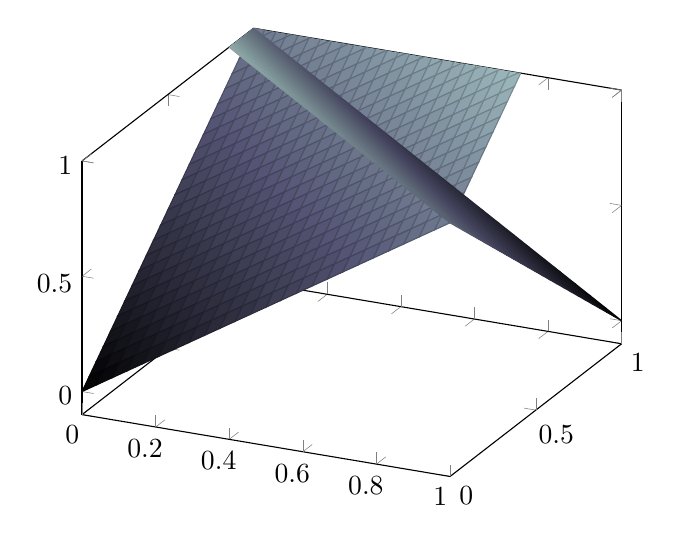
\begin{tikzpicture}
            %\draw[thick,->] (0,0,0) -- (1.5,0,0) node[right]{$x$};
            %\draw[thick,->] (0,0,0) -- (0,1.5,0) node[above]{$y$};
            %\draw[thick,->] (0,0,0) -- (0,0,1.5) node[left]{$z$};
            %\addplot3[
            \begin{axis}[domain = 0:1, zmax=1, colormap/bone]
                \addplot3[surf,name path = first,domain=0:1, domain y=0:1]
                {x + y};
                \addplot3[surf,name path = second,domain=0:1, domain y=0:1]
                {2-x-y};
                %\addplot[left color = black, right color = black!50, draw = none]
                %fill between[of = first and second];
            \end{axis}
        \end{tikzpicture}
    \end{center}
    \caption{Bounds of $z_{i,j}$}
\end{figure*}
From this graph we see the conditions of $z_{i,j}$, where it must be less than 
this. From this graph we can see that the bounds given in the above table show
that all $(x,z)$ that are feasible, under the constraints, satisfy this condition.
\FloatBarrier


%Looking at the objective function, we'll need to solve for the expectation value.
%\begin{align*}
%    \langle F(x)\rangle &= \left\langle\sum\limits_{(i,j)\in\mathcal{E}} w_{i,j}z_{i,j}\right\rangle\\
%           &= \sum\limits_{(i,j)\in\mathcal{E}} w_{i,j}\mathbf{Pr}(\mathsf{vertex\ within\ cut}) \\
%           &= \sum\limits_{(i,j)\in\mathcal{E}} w_{i,j}\frac12\\
%           &= \frac12 \cancelto{1}{\sum\limits_{(i,j)\in\mathcal{E}}w_{i,j}} \\
%           &= \frac12
%\end{align*}
%We can determine that $\mathbf{Pr}(\mathsf{vertx\ within\ cut}) = \frac12$ if
%we better define this as the probability that a vertex is on one side of a cut.
%This is clearly a bifrication problem and thus the value is $\frac12$.
%
%Since we can see that the expectation value, $\langle F(x)\rangle = \frac12$, 
%and thus we can conclude that $F(x)\geq \frac12\sum\limits_{(i,j)\in\mathcal{E}}w_{i,j}z_{i,j}$

\problem{2}
For the directed graph $G=(\mathcal{U,E})$, where $\mathcal{U}$ is the set of 
vertices and $\mathcal{E}$ is the set of directed edges, we want to partition 
$\mathcal{U}$ into two sets, $\mathcal{V}$ and $\mathcal{W}=\mathcal{U}/
\mathcal{V}$, in order to maximize the total weight of the edges going from 
$\mathcal{V}$ to $\mathcal{W}$ (edges $(i,j)$ with $i\in\mathcal{V}$ and 
$j\in\mathcal{W}$)

\begin{itemize}
    \item Give a randomized $\frac14$-approximation algorithm for this problem.
    \item Show that the following linear program is a relaxation of this problem.
\end{itemize}
\begin{align*}
    max & \sum\limits_{(i,j)\in\mathcal{E}} w_{i,j}z_{i,j}\\
    s.t.\hspace{1em}& z_{i,j} \leq x_i, \forall(i,j)\in \mathcal{E}\\
        & z_{i,j}\leq 1 - x_j, \forall(i,j)\in \mathcal{E}\\
        & 0 \leq x_i \leq 1, \forall i\in \mathcal{U}\\
        & 0 \leq z_{i,j} \leq 1, \forall (i,j)\in\mathcal{E}
\end{align*}
\begin{itemize}
    \item For the above linear program, give a randomized $\frac12$-approximation
          algorithm based on rounding $x_i\forall i\in\mathcal{U}$ to 1, with the
          probability of $\frac12x_i + \frac14$
\end{itemize}

\ppart{1}
For the $\frac14$ approximation we can look at the expectation value of the
function, we only need to consider $z_{i,j}$
\begin{align*}
    \langle z_{i,j} \rangle &= Pr(vertex\ within\ cut\wedge from\ i\ to\ j)\\
            & Pr(vertex\ within\ cut)Pr(from\ i\ to\ j)\\
            & \left(\frac12\right)\left(\frac12\right)\\
            & \frac14
\end{align*}
\ppart{2}
\FloatBarrier
For this we need to describe the original problem. We can say
\begin{align*}
    \max\hspace{2em} &\sum\limits_{(i,j)\in\mathcal{E}} w_{i,j}(1-x_i)x_j \\
    s.t. \hspace{2em}& x\in\{0,1\}
\end{align*}
We can similarly use an injective map to show that the LP (given) is a relaxation
of the above ILP.
\begin{figure*}[h!]
    \begin{center}
        \begin{tabular}{|c|c|c|c|}
            \hline
            $x_i$ & $x_j$ & ILP & LP\\
            \hline
            0 & 0 & 0 & 0\\
            \hline
            1 & 0 & 0 & 0\\
            \hline
            0 & 1 & 1 & 1\\
            \hline
            1 & 1 & 0 & 0\\
            \hline
        \end{tabular}
    \end{center}
\end{figure*}
\FloatBarrier
It is easy to see that in the ILP that any time $x_j=0$ or $x_i=1$ then
the objective function is 0. We can do the same thing by looking at the LP
constraints, showing that $z_{i,j}\leq x_i$ and $z_{i,j} \leq 1-x_j$. Similar to 
problem 1 we need both constraints. 

\ppart{3}
If we look back at our expectation values we can see that the probability that
$Pr(x\in\mathcal{V}) = \frac12$, and from here it is easy to see that the rounding
is $\frac12 x_i$ (given that it is bound between 0 and 1). We can then add the 
$\frac14$ approximation algorithm to get the result 


\end{document}
